% ============================================================
%  ANNEXES
% ============================================================

% ============================================================
%  ANNEXE 1 : SIMULATIONS HEC-RAS
% ============================================================
\chapter{Les simulations sur le Logiciel HEC-RAS pour le calcul de la lame d'eau sur le coursier}
\label{ann:hecras}

\section{Introduction}
\label{sec:ann1_intro}

La présente annexe regroupe les éléments détaillés de la modélisation unidimensionnelle réalisée sous le logiciel HEC-RAS (\textit{Hydrologic Engineering Center -- River Analysis System}) dans le cadre du dimensionnement hydraulique de l'évacuateur de crues du barrage Ahl Souss. Cette modélisation, dont les principes et les résultats synthétiques sont présentés à la section \ref{sec:murs_bajoyers} du chapitre \ref{chap:dim_theorique}, a pour objectif de déterminer le profil de la ligne d'eau le long du coursier pour les trois débits de crue retenus (périodes de retour 10, 100 et 1\,000 ans), afin d'en déduire la hauteur des murs bajoyers nécessaire à la contenance de l'écoulement.

\section{Mise en place du modèle HEC-RAS}
\label{sec:ann1_modele}

\subsection{Etapes de la détermination de la lame d'eau sur le coursier}
\label{subsec:ann1_geometrie}

La première étape pour les simulations, avant la création d'un nouveau projet, consiste à régler les unités sur le système international SI, et ce en faisant : « \textbf{Options -- Unit System -- System International} »

Puis, pour la création d'un nouveau projet, on suit le cheminement : « \textbf{File -- New project} » et on lui donne un titre après le choix de son emplacement.

L'option « \textbf{Geometric Data -- River Reach} » permet de dessiner la géométrie du coursier comme suit :

\begin{figure}[H]
    \centering
    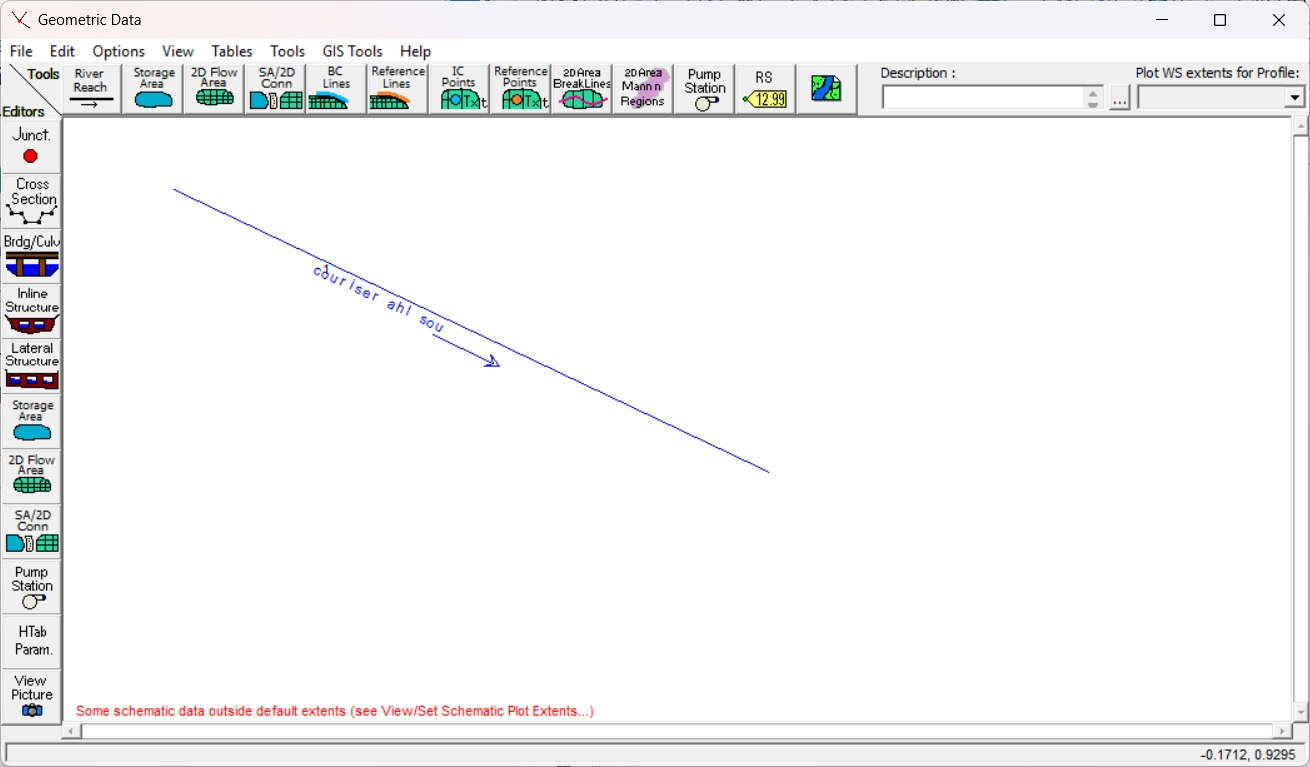
\includegraphics[width=0.85\textwidth]{figures/ann1_coursier_hecras.jpeg}
    \caption{Tracé schématique du coursier « coursier ahl sou » dans l'interface \textit{Geometric Data} de HEC-RAS (option \textit{River Reach})}
    \label{fig:ann1_coursier_hecras}
\end{figure}

L'étape suivante consiste à ajouter des sections transversales sur le coursier en cliquant sur « \textbf{Cross Section} » et on remplit les données concernant trois sections pour notre cas : section avale, section amont et la section de changement de la pente du coursier.

Les données à rentrer pour chaque section sont :
\begin{itemize}
    \item Les quatre coordonnées de la section (2 points niveau haut et 2 points niveau bas) ;
    \item La longueur séparant la section présente avec la section la plus proche en aval ;
    \item Les coefficients de Mannings prenant la valeur 0,014 pour le coursier construit en béton ;
    \item Les abscisses des stations rive gauche et rive droite ;
    \item Les coefficients d'expansion (0,3) et de contraction (0,1).
\end{itemize}

A noter que le logiciel commence toujours les sections de l'aval vers l'amont.

\begin{figure}[H]
    \centering
    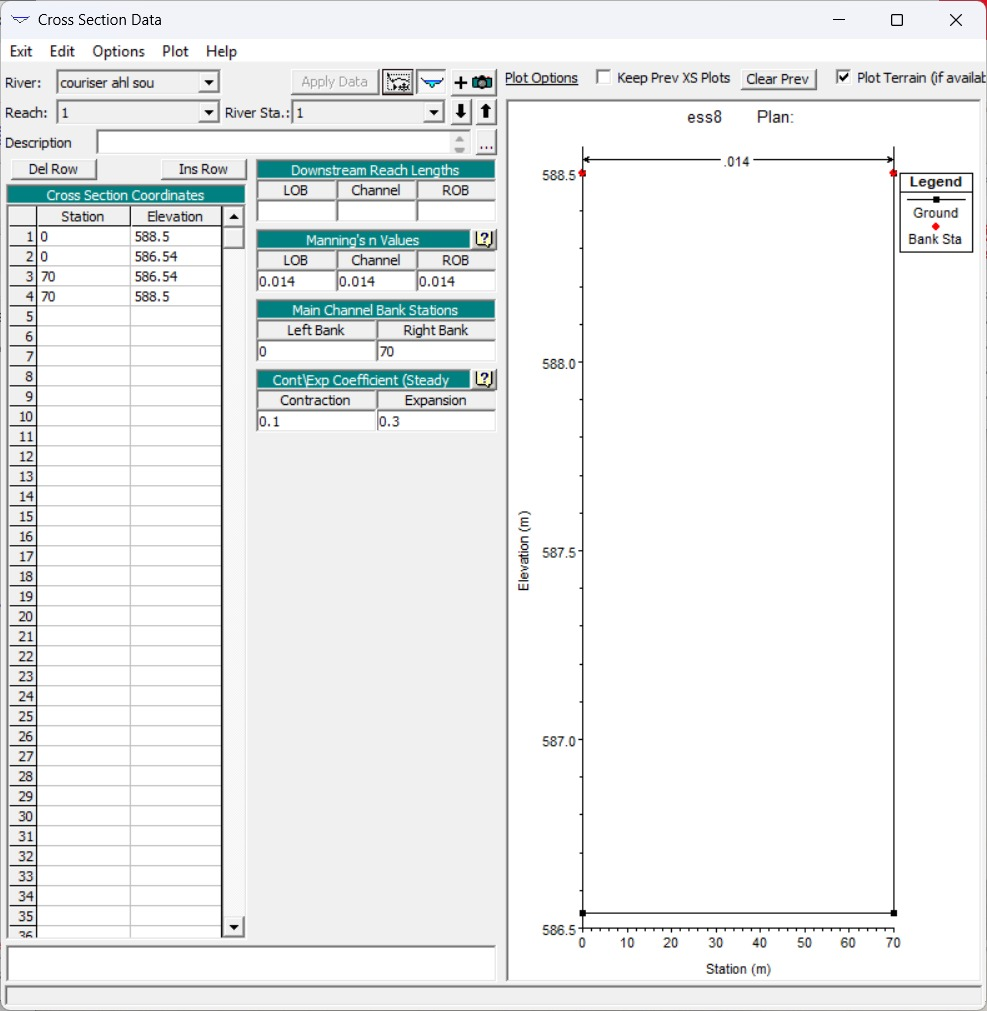
\includegraphics[width=\textwidth,height=0.42\textheight,keepaspectratio]{figures/ann1_section_aval.jpeg}\\[0.5em]
    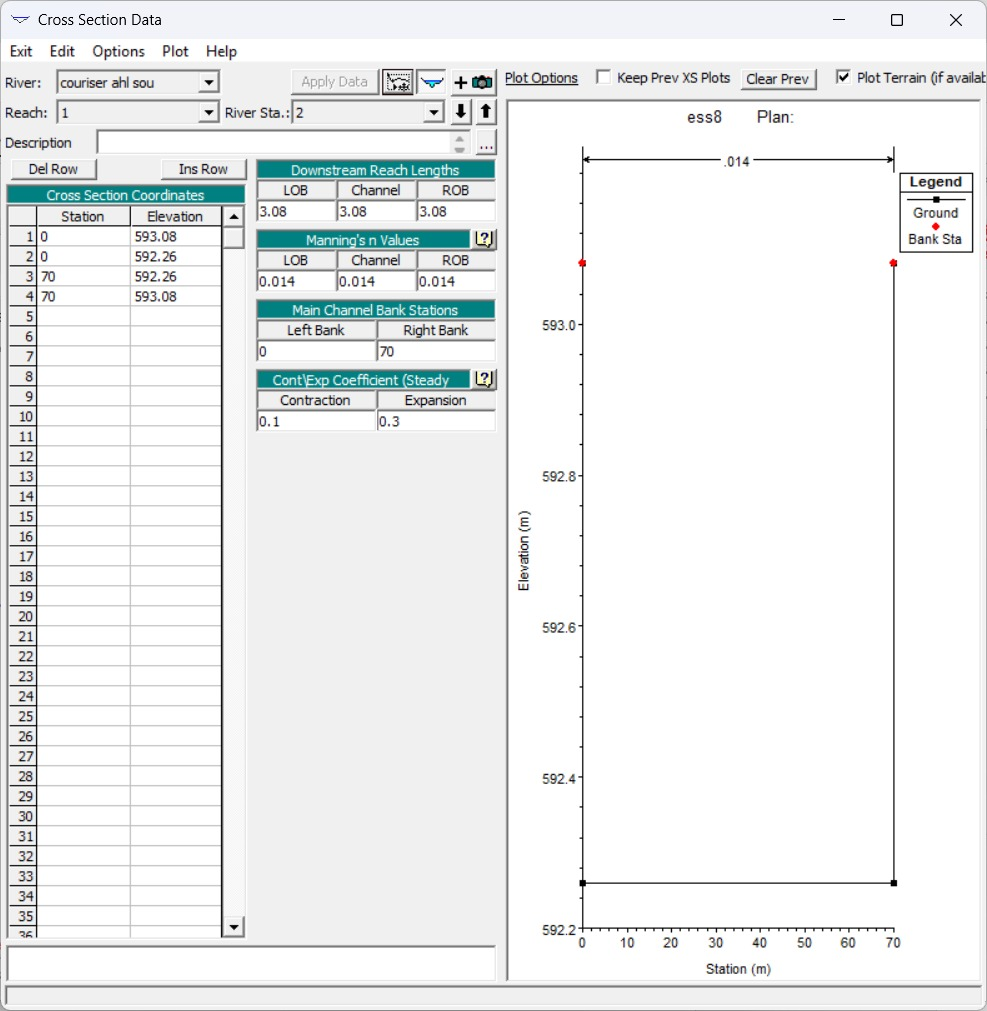
\includegraphics[width=\textwidth,height=0.42\textheight,keepaspectratio]{figures/ann1_section_changement_pente.jpeg}
\end{figure}

\clearpage

\begin{figure}[H]
    \centering
    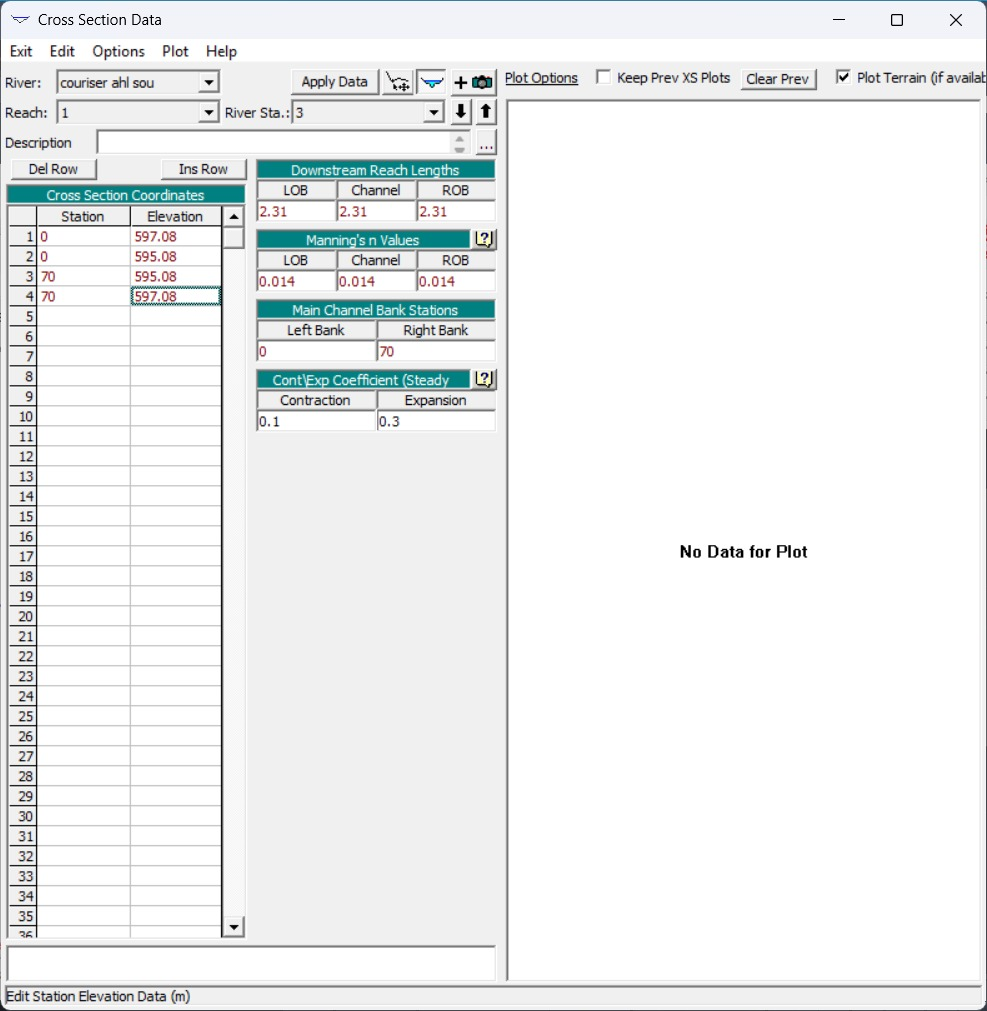
\includegraphics[width=\textwidth,height=0.75\textheight,keepaspectratio]{figures/ann1_section_amont.jpeg}
    \caption{Saisie des données des trois sections transversales du coursier dans HEC-RAS : section aval (RS\,=\,1), section de changement de pente (RS\,=\,2) et section amont (RS\,=\,3)}
    \label{fig:ann1_sections_transversales}
\end{figure}

Une fois que les données de chaque section sont remplies, on les conserve par « \textbf{Apply Data} ».

Pour ajouter d'autres sections transversales, afin de caractériser l'écoulement sur presque tout le coursier, on fait l'interpolation entre les sections pré-dessinées avec un pas de $2\,m$ en suivant « \textbf{Geometric Data -- Tools -- XS Interpolation} » :

\begin{figure}[H]
    \centering
    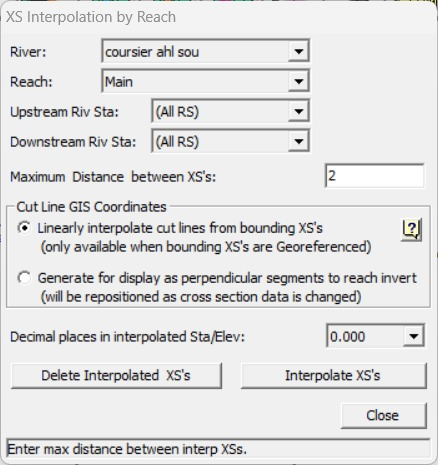
\includegraphics[width=0.65\textwidth]{figures/ann1_xs_interpolation.jpeg}
    \caption{Boîte de dialogue \textit{XS Interpolation by Reach} — interpolation des sections transversales avec un pas de 2\,m}
    \label{fig:ann1_xs_interpolation}
\end{figure}

Le résultat de l'interpolation est illustré par la figure suivante :

\begin{figure}[H]
    \centering
    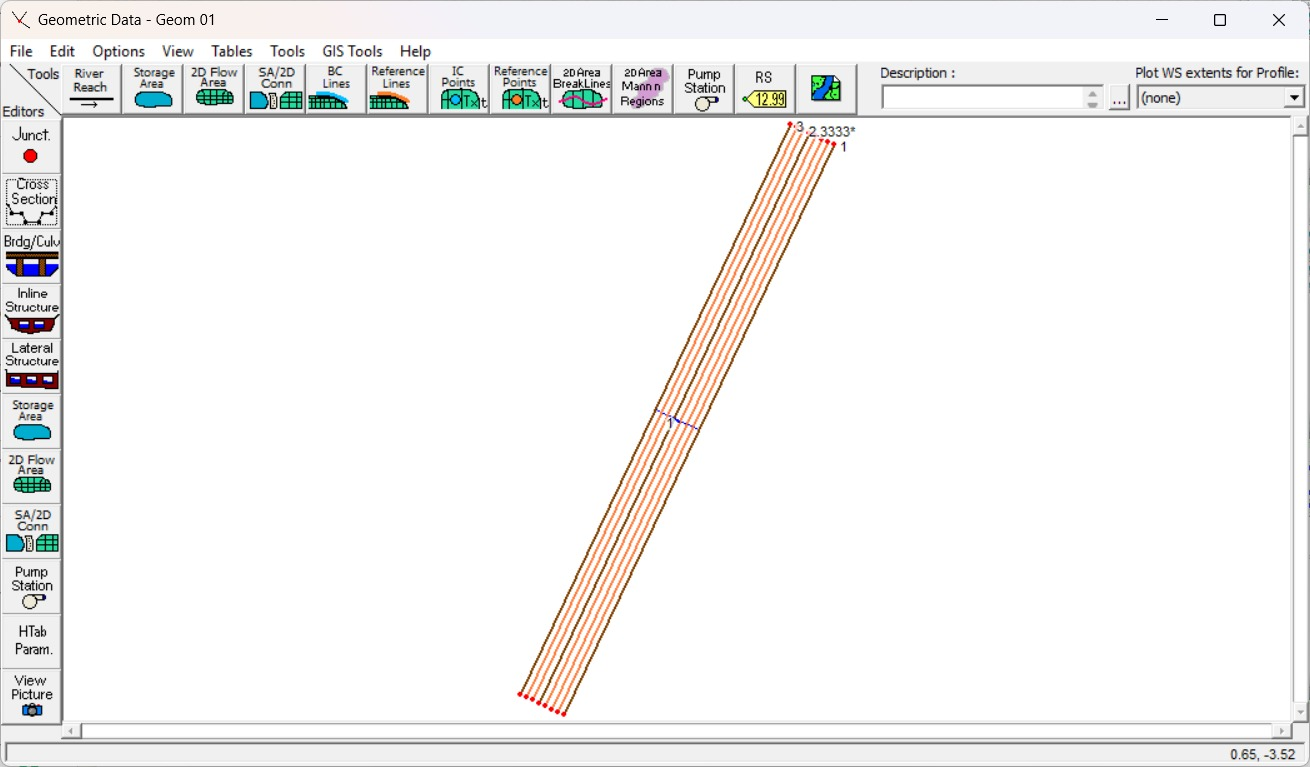
\includegraphics[width=0.85\textwidth]{figures/ann1_resultat_interpolation.jpeg}
    \caption{Visualisation des sections interpolées sur le coursier dans HEC-RAS}
    \label{fig:ann1_sections_interpolees}
\end{figure}

L'étape suivante consiste à entrer le débit de projet au logiciel et lui fixer les conditions aux limites.

Le débit de projet est inséré dans « \textbf{Steady Flow Data} » :

\begin{figure}[H]
    \centering
    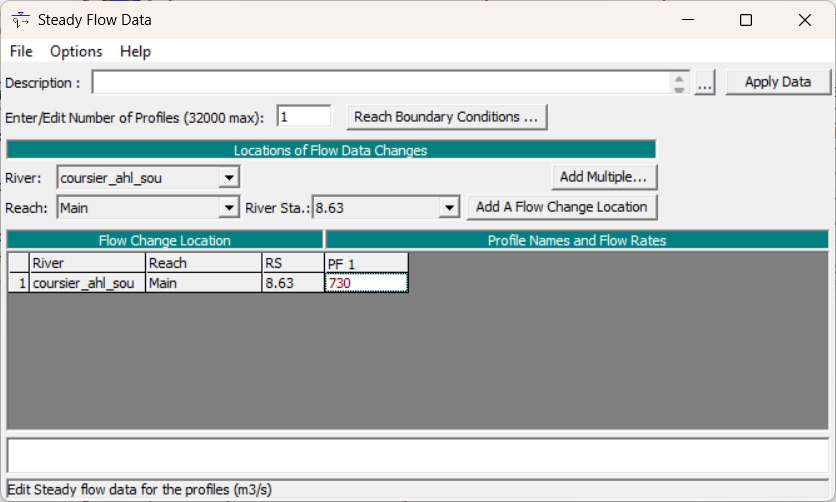
\includegraphics[width=0.85\textwidth]{figures/ann1_steady_flow_data.jpeg}
    \caption{Insertion du débit de projet et des conditions aux limites dans HEC-RAS (\textit{Steady Flow Data})}
    \label{fig:ann1_steady_flow}
\end{figure}

Les conditions aux limites sont insérées dans « \textbf{Steady Flow Data -- Reach Boundary Conditions} » en considérant la profondeur critique comme condition amont et la pente 18\,\% comme condition avale :

\begin{figure}[H]
    \centering
    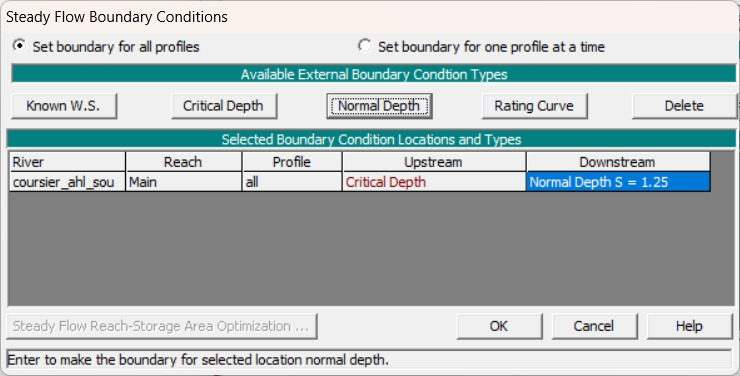
\includegraphics[width=0.85\textwidth]{figures/ann1_boundary_conditions.jpeg}
    \caption{Choix des conditions aux limites dans \textit{Steady Flow Boundary Conditions} : profondeur critique en amont, pente normale ($S = 1{,}25$) en aval}
    \label{fig:ann1_boundary_conditions}
\end{figure}

La dernière étape concerne l'exécution de la simulation qui consiste à fixer le régime de l'écoulement (fluvial ou torrentiel) et ce à travers « \textbf{Steady Flow Analysis} ». HEC-RAS donne la possibilité de le laisser lui-même déterminer le régime de l'écoulement en le fixant sur « \textbf{Mixed} ». L'exécution de la simulation se fait par « \textbf{Compute} » :

\begin{figure}[H]
    \centering
    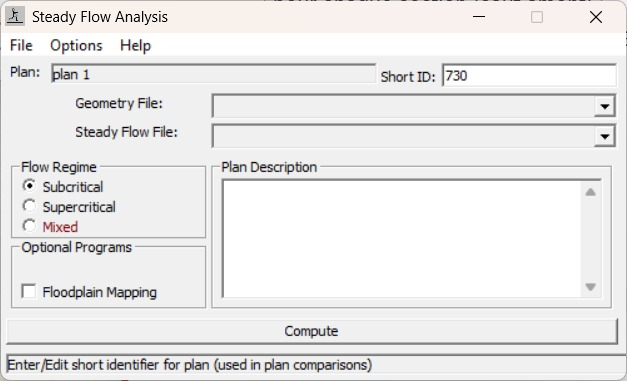
\includegraphics[width=0.75\textwidth]{figures/ann1_steady_flow_analysis.jpeg}
    \caption{Exécution de la simulation du projet HEC-RAS (\textit{Steady Flow Analysis}, régime Mixed)}
    \label{fig:ann1_steady_flow_analysis}
\end{figure}

Après quelques secondes, la simulation s'effectue avec réussite. Dès lors les résultats (Courbes, Dessins 2D, Tableaux\ldots) sont disponibles à visualiser.

\begin{figure}[H]
    \centering
    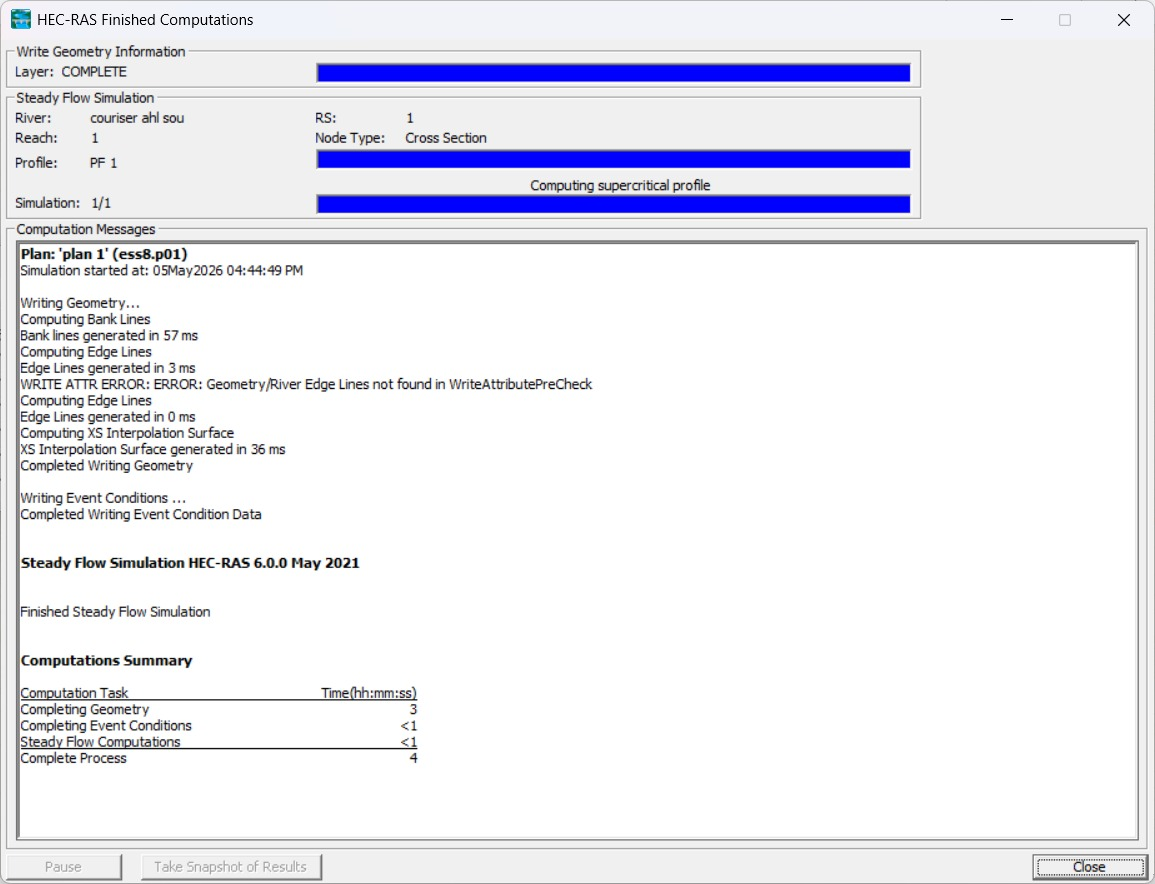
\includegraphics[width=0.92\textwidth]{figures/ann1_fin_simulation.jpeg}
    \caption{Interface de la fin de la simulation HEC-RAS (\textit{HEC-RAS Finished Computations})}
    \label{fig:ann1_finished_computations}
\end{figure}

% ============================================================
%  ANNEXE 2 : TABLEAUX DE CALCUL ET COURBES DE REMOUS
% ============================================================
\chapter{Les tableaux de calcul de la lame d'eau et les courbes de remous}
\label{ann:remous}

La présente annexe regroupe les tableaux complets de calcul de la courbe de remous établis par la méthode des pas dans le tableur Excel, pour chacun des trois débits de projet retenus ($Q_{10}$, $Q_{100}$ et $Q_{1\,000}$). Pour le débit millénaire $Q_{1\,000}$, le profil de la ligne d'eau est également représenté graphiquement.

% --- Q10 ---
\section{Tableau de calcul de la courbe de remous --- $Q_{10} = 175{,}11$ m³/s}
\label{sec:ann2_remous_q10}

\begin{figure}[H]
    \centering
    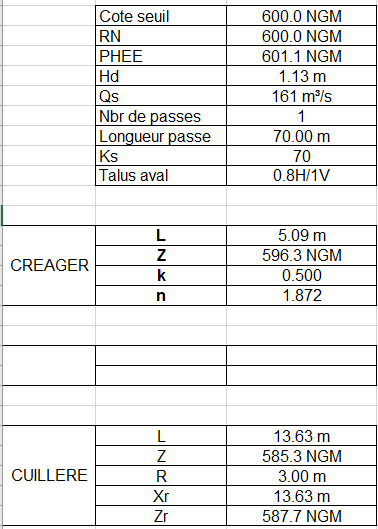
\includegraphics[width=0.65\textwidth]{figures/ann2_params_q10.png}
    \caption{Paramètres généraux de calcul pour $Q_{10} = 175{,}11$ m³/s : caractéristiques du seuil Creager et de la cuillère saut de ski}
    \label{fig:ann2_params_q10}
\end{figure}

\begin{figure}[H]
    \centering
    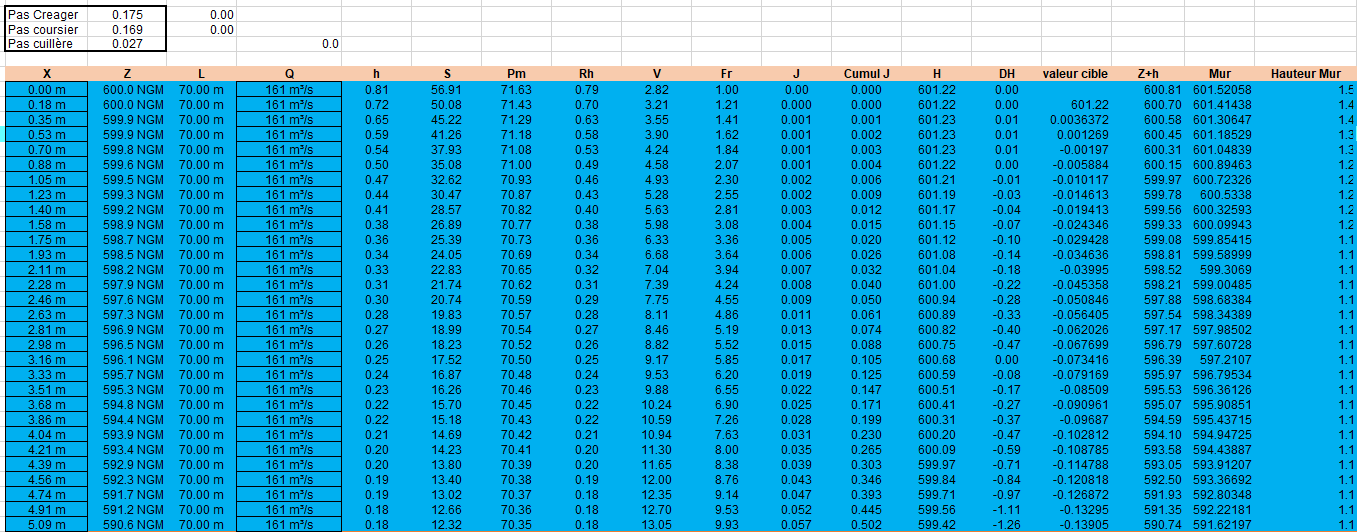
\includegraphics[width=\textwidth]{figures/ann2_seuil_q10.png}
    \caption{Tableau de calcul de la lame d'eau sur le seuil Creager — débit décennal $Q_{10} = 161$ m³/s (pas Creager\,=\,0,175\,m, pas coursier\,=\,0,169\,m, pas cuillère\,=\,0,027\,m)}
    \label{fig:ann2_seuil_q10}
\end{figure}

\begin{figure}[H]
    \centering
    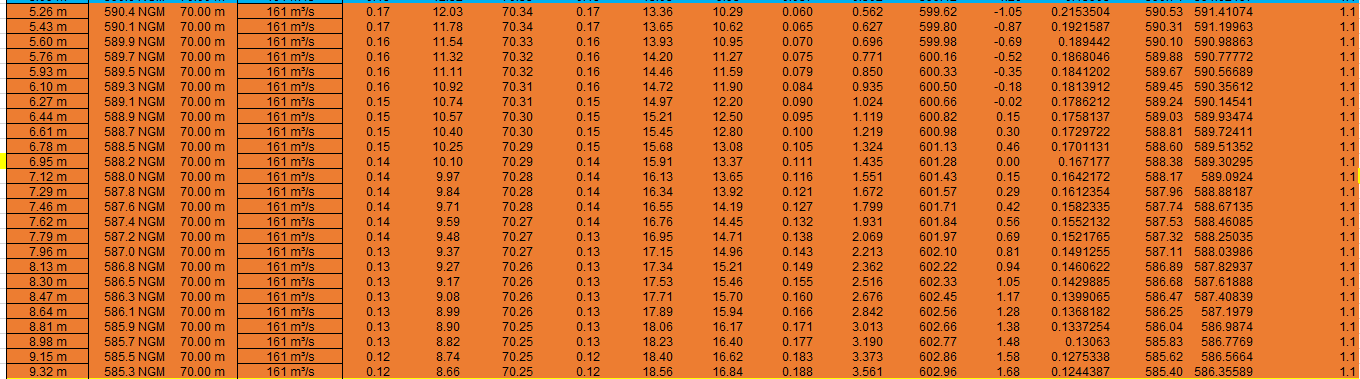
\includegraphics[width=\textwidth]{figures/ann2_coursier_q10.png}
    \caption{Tableau de calcul de la lame d'eau sur le coursier — débit décennal $Q_{10} = 161$ m³/s}
    \label{fig:ann2_coursier_q10}
\end{figure}

\begin{figure}[H]
    \centering
    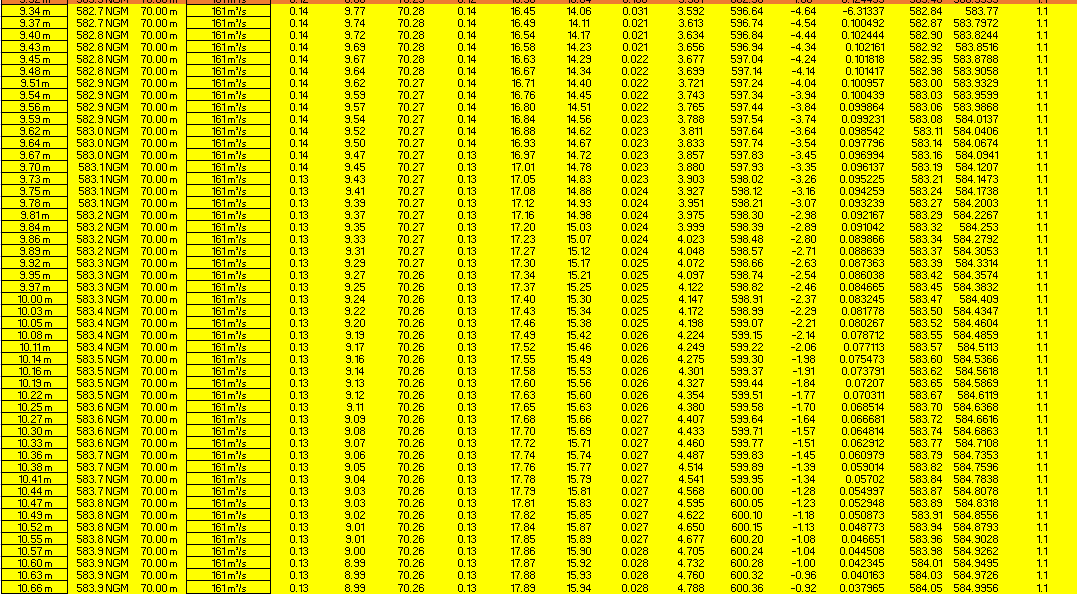
\includegraphics[width=\textwidth]{figures/ann2_cuillere_q10.png}
    \caption{Tableau de calcul de la lame d'eau sur la cuillère saut de ski — débit décennal $Q_{10} = 161$ m³/s}
    \label{fig:ann2_cuillere_q10}
\end{figure}

% --- Q100 ---
\section{Tableau de calcul de la courbe de remous --- $Q_{100} = 507{,}54$ m³/s}
\label{sec:ann2_remous_q100}

\begin{figure}[H]
    \centering
    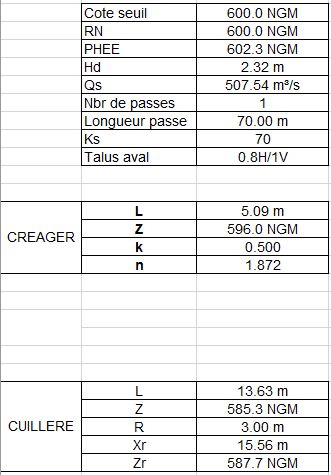
\includegraphics[width=0.65\textwidth]{figures/ann2_params_q100.png}
    \caption{Paramètres généraux de calcul pour $Q_{100} = 507{,}54$ m³/s : caractéristiques du seuil Creager et de la cuillère saut de ski}
    \label{fig:ann2_params_q100}
\end{figure}

\begin{figure}[H]
    \centering
    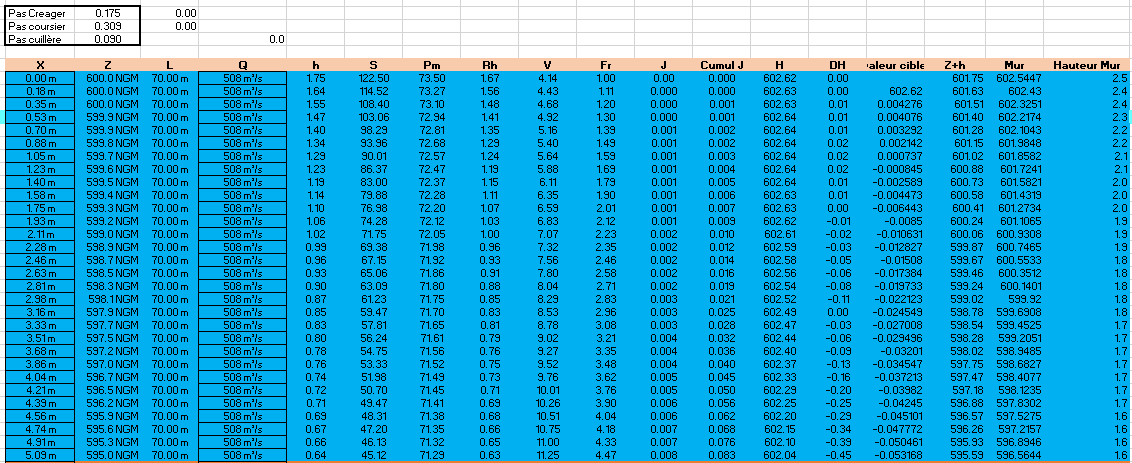
\includegraphics[width=\textwidth]{figures/ann2_seuil_q100.png}
    \caption{Tableau de calcul de la lame d'eau sur le seuil Creager — débit centennal $Q_{100} = 507{,}54$ m³/s}
    \label{fig:ann2_seuil_q100}
\end{figure}

\begin{figure}[H]
    \centering
    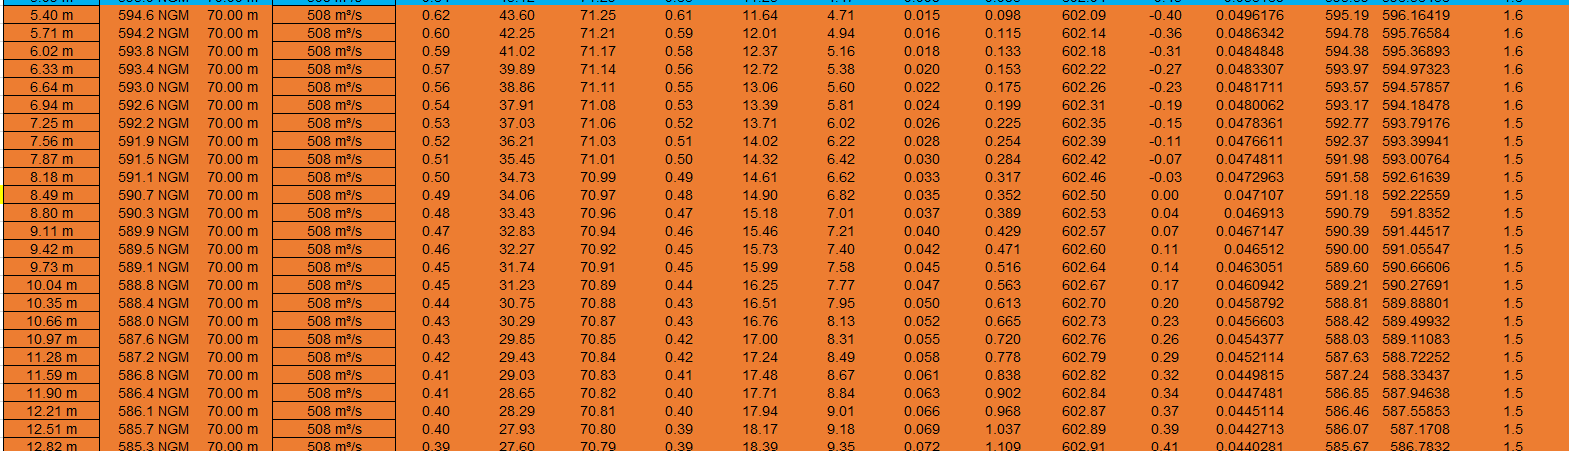
\includegraphics[width=\textwidth]{figures/ann2_coursier_q100.png}
    \caption{Tableau de calcul de la lame d'eau sur le coursier — débit centennal $Q_{100} = 507{,}54$ m³/s}
    \label{fig:ann2_coursier_q100}
\end{figure}

\begin{figure}[H]
    \centering
    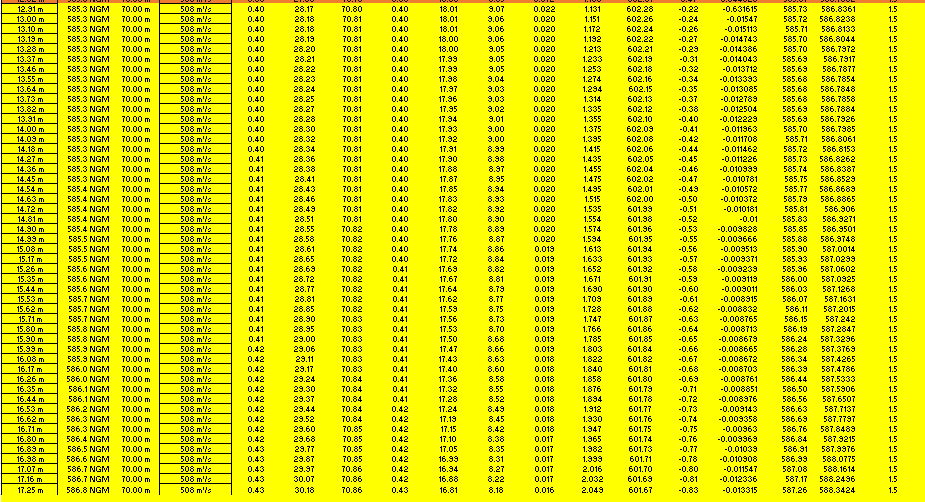
\includegraphics[width=\textwidth]{figures/ann2_cuillere_q100.png}
    \caption{Tableau de calcul de la lame d'eau sur la cuillère saut de ski — débit centennal $Q_{100} = 507{,}54$ m³/s}
    \label{fig:ann2_cuillere_q100}
\end{figure}

% --- Q1000 ---
\section{Tableau de calcul de la courbe de remous et graphe --- $Q_{1\,000} = 794{,}93$ m³/s}
\label{sec:ann2_remous_q1000}

\begin{figure}[H]
    \centering
    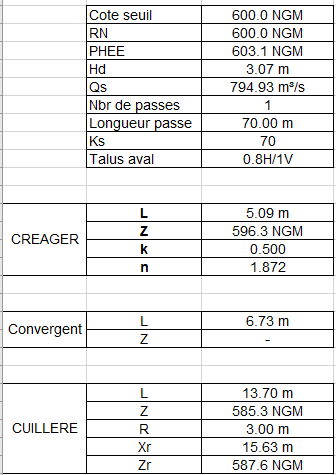
\includegraphics[width=0.65\textwidth]{figures/ann2_params_q1000.png}
    \caption{Paramètres généraux de calcul pour $Q_{1\,000} = 794{,}93$ m³/s : caractéristiques du seuil Creager et de la cuillère saut de ski}
    \label{fig:ann2_params_q1000}
\end{figure}

\begin{figure}[H]
    \centering
    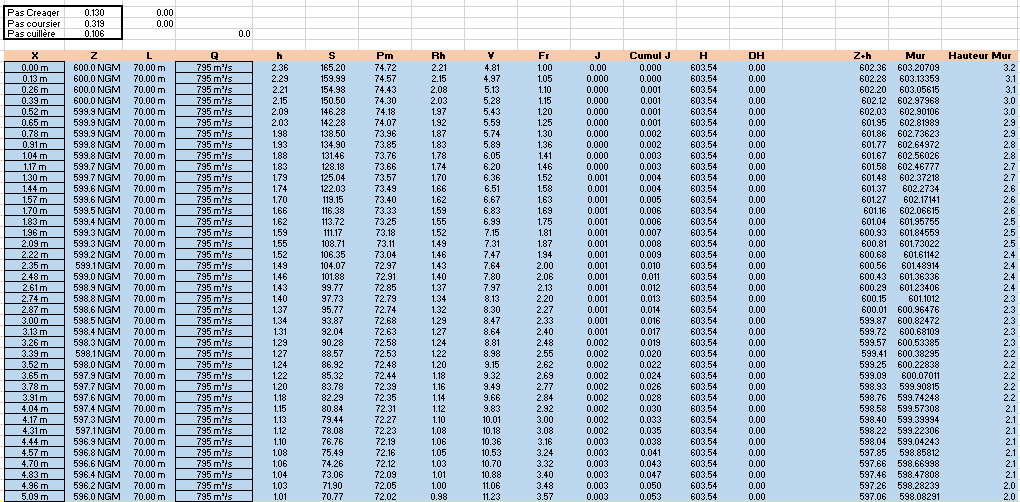
\includegraphics[width=\textwidth]{figures/ann2_seuil_q1000.png}
    \caption{Tableau de calcul de la lame d'eau sur le seuil Creager — débit millénaire $Q_{1\,000} = 794{,}93$ m³/s}
    \label{fig:ann2_seuil_q1000}
\end{figure}

\begin{figure}[H]
    \centering
    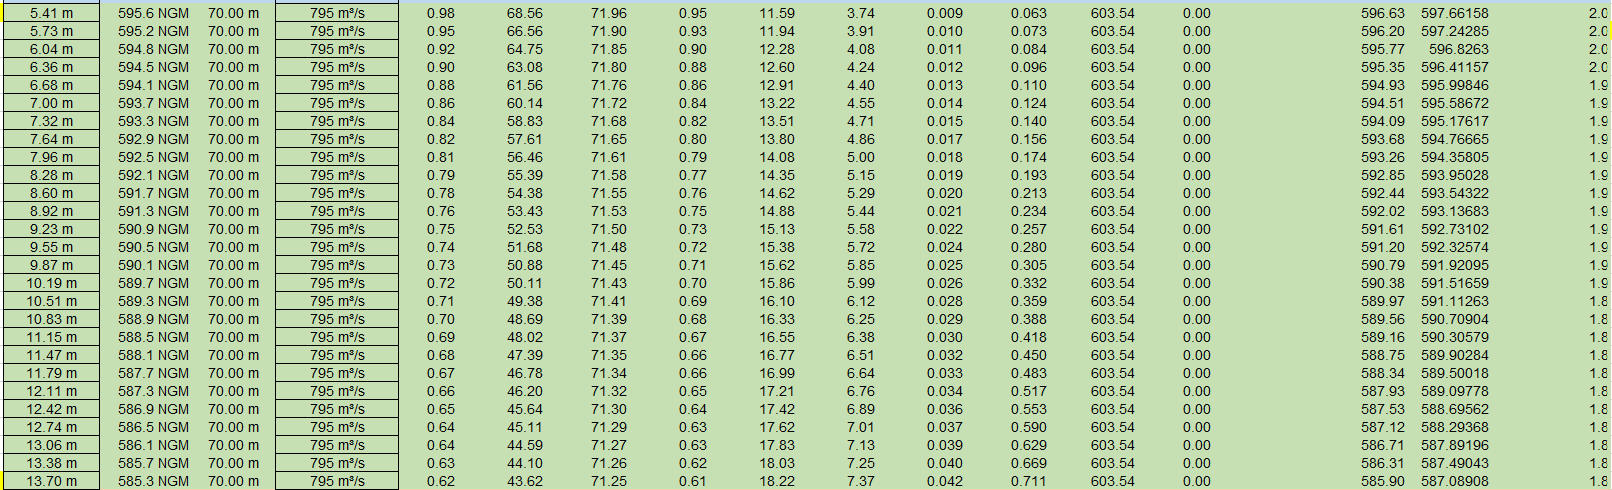
\includegraphics[width=\textwidth]{figures/ann2_coursier_q1000.png}
    \caption{Tableau de calcul de la lame d'eau sur le coursier — débit millénaire $Q_{1\,000} = 794{,}93$ m³/s}
    \label{fig:ann2_coursier_q1000}
\end{figure}

\begin{figure}[H]
    \centering
    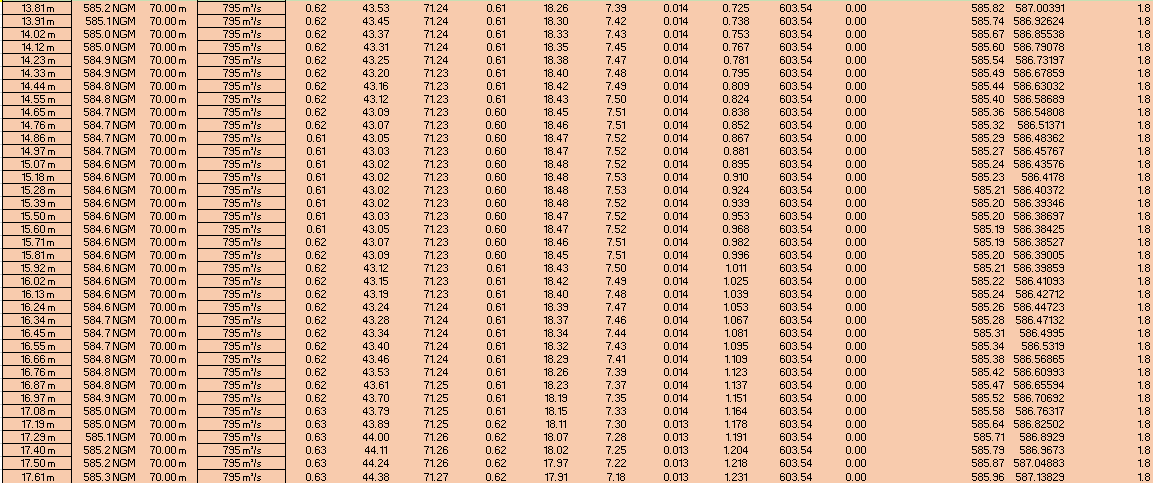
\includegraphics[width=\textwidth]{figures/ann2_cuillere_q1000.png}
    \caption{Tableau de calcul de la lame d'eau sur la cuillère saut de ski — débit millénaire $Q_{1\,000} = 794{,}93$ m³/s}
    \label{fig:ann2_cuillere_q1000}
\end{figure}

\begin{figure}[H]
    \centering
    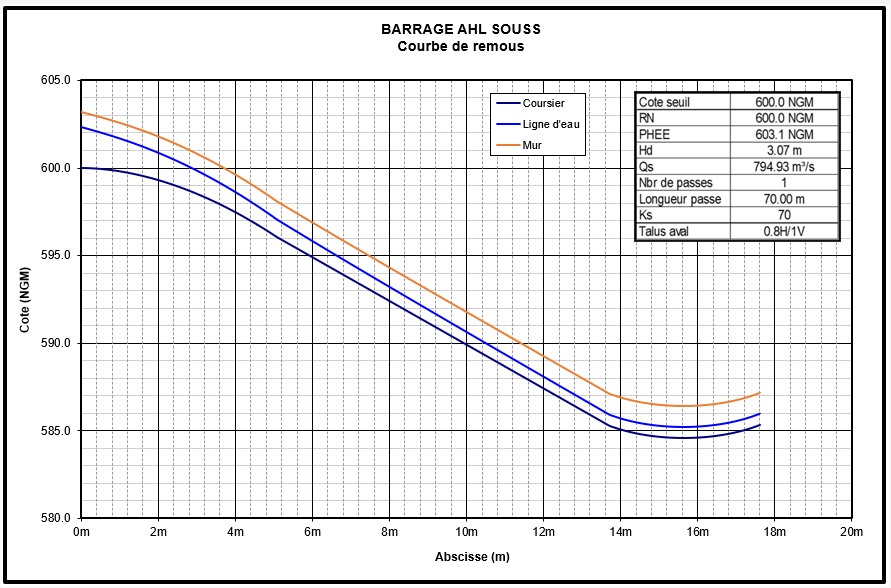
\includegraphics[width=\textwidth]{figures/courbe_remous.png}
    \caption{Courbe de remous — profil de la ligne d'eau le long du coursier pour $Q_{1\,000} = 794{,}93$ m³/s}
    \label{fig:ann2_courbe_remous_q1000}
\end{figure}
